\chapter{MLP-SOM supervised model experiment}
\label{chap:mlp-som}

In this chapter, we focused on the development and testing of a new method that involves Self-organising map representation, positions of prototypes of inputs, as auxiliary information used in training of Multi-layer perceptron. Yet, we used a simple supervised setup to find ways of usage of such auxiliary information. We designed an experiment for testing this method and compared the performance of MLP with and without additional structural information SOM map. This experiment was designed with a table dataset containing attributes acquired from samples of several wine species


\section{Motivation}
Self-organizing maps are able to naturally cluster data and project them into low-dimensional representation - a map. This is determined by neurons also called prototypes. Each prototype has its weights, which are adjusted during unsupervised training to represent a subset of the input data samples. The weights of the prototype have the same dimension $n$ as input data. The position of the prototype on the SOM map is determined by two coordinates, row and column since a two-dimensional map is used. SOM is most well-trained when one prototype represents inputs mostly from the same class.

We aimed to develop an idea, to use these prototypes during learning of the supervised model as a supportive element. We used distance on the SOM map of SOM two prototypes representing two inputs as an approximation of the difference of the inputs. By that, we helped the network to learn from information about the difference between two samples.

\newpage
\section{SOM based loss propositions}
We were considering several forms of SOM-based loss. In each, we use the computation of Euclidean distance of two vectors of size $2$ (positions on the map of prototypes). The computation of Euclidean distance $D_E$ of vectors $x$ and $z$ of size $2$  is shown in equation \ref{eq-dist}.

\begin{equation}
    D_E(x, z) = \sqrt{\sum_{i=1}^{2} {(x_i - z_i)}^2}
    \label{eq-dist}
\end{equation}
\bigskip

\subsection{Prototype distance SOM based loss}
\label{loss-prop1}
The first SOM loss form we considered was based on a pair of data points $x$ and $z$. They could be from the same or different class. We found their prototypes $p(x)$ and $p(z)$ as predictions of data points, based on competitive principle. This notation means the position of the prototype in a two-dimensional grid. Then we computed their distance $D_E(p(x), p(z))$ using equation \ref{eq-dist}. If data points were from the same class, we wanted the distance close to zero. If the second data point was from a different class, the distance should have been high. Our proposed SOM loss is then defined by the previous equation \ref{eq-dist}.

\begin{figure}[h!]
    \centering
    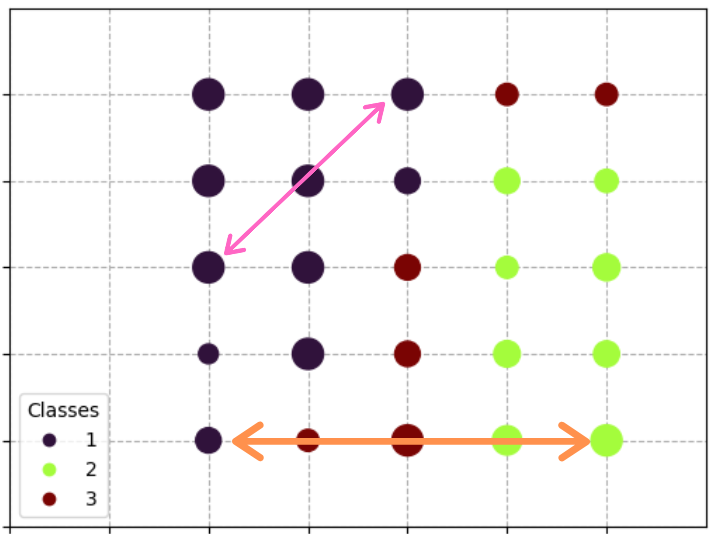
\includegraphics[width=0.5\textwidth]{figs/som-with-distances.png}
    \caption{SOM map with denoted Euclidean distances of selected neurons}
    \label{fig:som-with-distances}
\end{figure}

In figure \ref{fig:som-with-distances}, we show Euclidean distances of pairs of selected winners on the SOM 2-dimensional map. Distances are denoted as arrows. The orange arrow shows the Euclidean distance of the SOM map of two prototypes from incongruent classes, while the pink arrow in Euclidean distance between two prototypes from the congruent class.

The drawback of this definition was, that we would need to somehow discriminate which distances are small enough to represent the same class and which are big enough to represent data points from different class and we do not know the upper bound of value of such loss. The threshold would need to be set experimentally, based on data.

\subsection{Congruent and incongruent distance SOM-based loss}
\label{loss-final}
In a supervised setup, since we know all desired labels in the training set, we can fix the drawback from section \ref{loss-prop1} using normalization, for which we need to compute two distances. The first distance was the mean distance of pairs of samples from the same (congruent) class $D_C$, and the second was the mean distance of pairs of samples from different (incongruent) classes $D_I$. We used triplets of inputs to compute the distances. Then we computed the mean distances $D_C$ and $D_I$. The first sample of triplet was denoted as $x$, the second sample $z$ was from congruent class to $x$ and the third sample $\xi$ was from incongruent class. Distances were computed based on equations \ref{eq-dist3}, \ref{eq-dist4}. Then, we computed normalized distance $D$ as described in equation \ref{eq-som-loss}.

\begin{equation}
    D_C = \frac{1}{n} \sum_i^n D_E(g(x_i, \tau), g(z_i, \tau)) 
    \label{eq-dist3}
\end{equation}

\begin{equation}
    D_I = \frac{1}{n} \sum_i^n D_E(g(x_i, \tau), g(\xi_i, \tau)) 
    \label{eq-dist4}
\end{equation}

\begin{equation}
    D = \frac{D_I - D_C}{D_I + D_C}
    \label{eq-som-loss}
\end{equation}

In the following table \ref{tab-dists}, different values of distances were investigated. As a result, we can see that the proposed distance $D$ resolves all cases when distances of congruent and incongruent samples are high or low.
We can explain these cases. The first and last cases are when distances are really close and the loss is 0, so it has no information value because distances give no information about the sample being closer to the original sample, whether congruent or incongruent. In case 2, the result is positive and it is a good case when the incongruent sample is far from the original and congruent is close to the original. In the third case, loss is negative and this is the case when distances are opposite as they should be. We decided to rescale this loss with absolute values from interval $(0, 1)$. The equation \ref{rescale-som-loss} explains this scaling and provides a loss function that acquires only non-negative and loss is lower when the distance of congruent samples is small and of incongruent is high. Loss is high if the mistake in distance is high.

\begin{equation}\label{rescale-som-loss}
\begin{split}
J_S(\tau) = \frac{1}{2}  - \frac{1}{2} \cdot D = \frac{1}{2}\Biggl(1 - \frac{D_I - D_C}{D_I + D_C}\Biggr) = \\[20pt]  
\frac{1}{2}(\frac{D_I + D_C}{D_I + D_C} - \frac{D_I - D_C}{D_I + D_C}) = 
\frac{1}{2}(\frac{2D_C}{D_I + D_C}) = \frac{D_C}{D_I + D_C}
\end{split}
\end{equation}


\begin{table}[ht]
    \centering
    \begin{tabular}{|rr|rr|rr|rr|}
    \hline
    \multicolumn{2}{|c|}{$D_I$}            & \multicolumn{2}{c|}{$D_C$}            & \multicolumn{2}{c|}{$D$}                & \multicolumn{2}{c|}{$J_S$}                \\ \hline
    
    \multicolumn{1}{|r|}{1000} & high & \multicolumn{1}{r|}{1000} & high & \multicolumn{1}{r|}{0}      & middle & \multicolumn{1}{r|}{0.5}    & middle \\ \hline
    
    \multicolumn{1}{|r|}{1000} & high & \multicolumn{1}{r|}{1}    & low  & \multicolumn{1}{r|}{0.998}  & high   & \multicolumn{1}{r|}{0.0009} & low    \\ \hline
    \multicolumn{1}{|r|}{1}    & low  & \multicolumn{1}{r|}{1000} & high & \multicolumn{1}{r|}{-0.998} & low    & \multicolumn{1}{r|}{0.99}   & high   \\ \hline
    \multicolumn{1}{|r|}{1}    & low  & \multicolumn{1}{r|}{1}    & low  & \multicolumn{1}{r|}{0}      & middle & \multicolumn{1}{r|}{0.5}    & middle \\ \hline
    \end{tabular}
    \caption{Distance function $D$ in all possible cases}
    \label{tab-dists}
\end{table}

\subsection{Supervised loss and SOM loss combined}
We proposed combined loss $Loss$ which combines supervised loss $S$ defined in equation \ref{eq:mt-som-sup} as mean squared error of model prediction and desired output $\hat{y}$ and $J_S$ multiplied by hyperparameter $\kappa$, as shown in equation \ref{comb-loss}.
Parameter $\kappa$ is linearly ramped down during the training from maximum value to zero. Value of $\kappa$ in epoch $t$ is denoted as $\kappa(t)$.

\begin{equation}
	S(\theta) = \frac{1}{n} \sum_i^n  ||g(x_i, \theta), \hat{y}||^2
	\label{eq:mt-som-sup}
\end{equation} 

\begin{equation}
    Loss(\theta) = S(\theta) + \kappa(t) \cdot J_S(\tau)
    \label{comb-loss}
\end{equation}

\section{Experiment}
We designed an experiment to investigate how proposed $\text{SOM-Sup-Loss}$ influences the learning abilities of the supervised model in the task of classification into three classes. We compare the baseline supervised model - Multi-layer perceptron with mean squared error loss and the same model in setup with $\text{SOM-Sup-Loss}$. We used pre-trained SOM for determining distances of samples and for computation of $\text{SOM-Sup-Loss}$.

\subsection{Wine dataset}
We chose a table dataset called the Wine dataset. These data are the results of a chemical analysis of wines grown in the same region in Italy but derived from three different cultivars. The analysis determined the quantities of 13 constituents found in each of the three types of wines. Data was vectors of length $13$ from three classes defined by the three cultivars. The dataset contained $59$, $71$ and $48$ training samples per class. \cite{misc_wine_109} 
We chose the table dataset rather than the image dataset to accelerate our research, since image datasets are much more demanding in terms of resources and therefore take much longer training time.

We split the dataset into training and testing parts such that the test dataset contained approximately $25\%$ of samples, and each class had the same number of samples in the testing dataset. That meant $15$ samples from each class. Other $75\%$ of data created training dataset. In this training dataset, data were reorganized in the way that each sample was paired with another sample from the same class and another sample from a different class. The final training dataset was composed of $6650$ triplets. We refer to the first sample of triplet as the original sample, the second sample as a congruent sample, and the third sample as an incongruent sample.

\subsection{Baseline}
\label{sup-baseline}
As the baseline, we chose a Multi-layer perceptron (MLP) trained in a fully supervised setup. We used the mean squared error loss function. We started with architecture with 4 layers with few tenths of neurons in each layer and sigmoid activation functions. Such a model was too complex for this tiny dataset and after the selection of appropriate learning rate parameter, it was able to train on the dataset and discriminate classes with $100\%$ test accuracy. 

Since we wanted to show the advantages of the model that uses SOM, we decreased the complexity of the architecture. We chose architecture with only one hidden layer, with $15$ neurons and a sigmoid activation function. The complete structure of layers is shown in table \ref{mlp=layers}. MLP with this architecture was not able to achieve $100\%$ testing accuracy on the dataset, so it was suitable for our experiment.


\begin{table}[ht]
    \centering
    \begin{tabular}{ |c|c|c|} 
     \hline
            Layer & Number of neurons & Activation function\\
            \hline
            input fully connected & 13 &  - \\
            hidden fully connected & 15 & sigmoid  \\
            output fully connected  & 3 & softmax \\
     \hline
    \end{tabular}
    \caption{Architecture of MLP}
    \label{mlp=layers}
\end{table}

The model was implemented using PyTorch library \cite{pytorch} with default weight initialization.
Other parameters of MLP were learning rate and optimizer type. \textbf{Learning rate} was set to $0.0001$ and \textbf{Adam optimizer} was used. 




\subsection{MLP-SOM model}
For our MLP-SOM model, we used the same architecture \ref{mlp=layers} as for the baseline. We used combined loss described in \ref{comb-loss}. We were considering several ways how to include SOM information in MLP. We tried to train SOM in each epoch of training MLP, but it led to overfit in SOM, since SOM inputs did not change and the dataset is low in complexity and number of samples. To resolve this problem we rather used pre-trained SOM. We pre-trained SOM on data samples and used information from SOM predictions in the unsupervised part of loss \ref{comb-loss}. 


\subsubsection{Pre-trained SOM}
\label{pretrained-som}
SOM topology consisted of $5 \times 5$ neurons. SOM hyperparameters were learning rate $\alpha$ which was linearly ramped down from maximal value $0.3$ to $0$. As a neighbor function in SOM training Gaussian function with parameter $\sigma$ was used. This parameter was linearly ramped down from value $2.5$ to $0$. SOM was trained for $20$ epochs and the map representation is shown in figure \ref{fig:somka}.
SOM metrics at the end of training were quantization error = $682.59$, winner discrimination = $100 \%$, entropy = $4.37$. Change of these metrics in time ($20$ epochs) are shown in graphs in figure \ref{fig:som-metrices}.


\begin{figure}[h!]
    \centering
    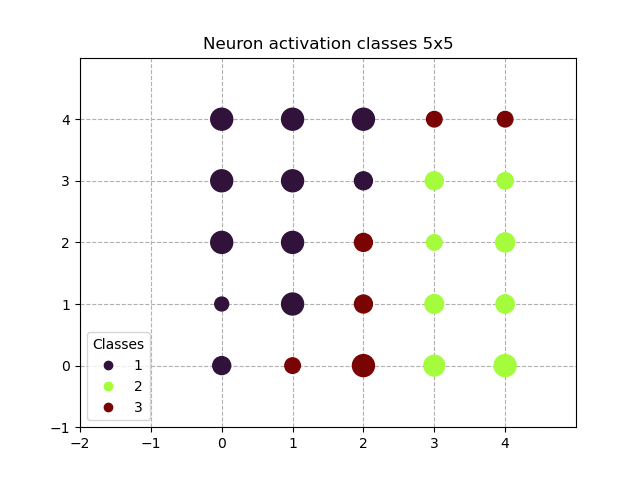
\includegraphics[width=0.8\textwidth]{figs/som1710255005.5160155.png}
    \caption{SOM used for Wine experiment}
    \label{fig:somka}
\end{figure}

SOM we use is well organized, as shown in figure \ref{fig:som}. We can see three separate clusters corresponding to three classes in the dataset. There are two outlier red prototypes from class 3 not connected to the rest of the prototypes from class 3 in the right upper corner of the map. From SOM metrics in figure \ref{fig:som-metrices}, we can infer that the quantization error has a decreasing trend, which is good. Winner discrimination is between $96\%$ and $100\%$ which means at least $96\%$ of neurons were chosen as the prototype for some datapoint, so we use almost all and in the last few epochs all the parameters of the model to encode a subset of input samples. Entropy has an increasing trend, which is also correct.


\begin{figure}[h!]
    \centering
    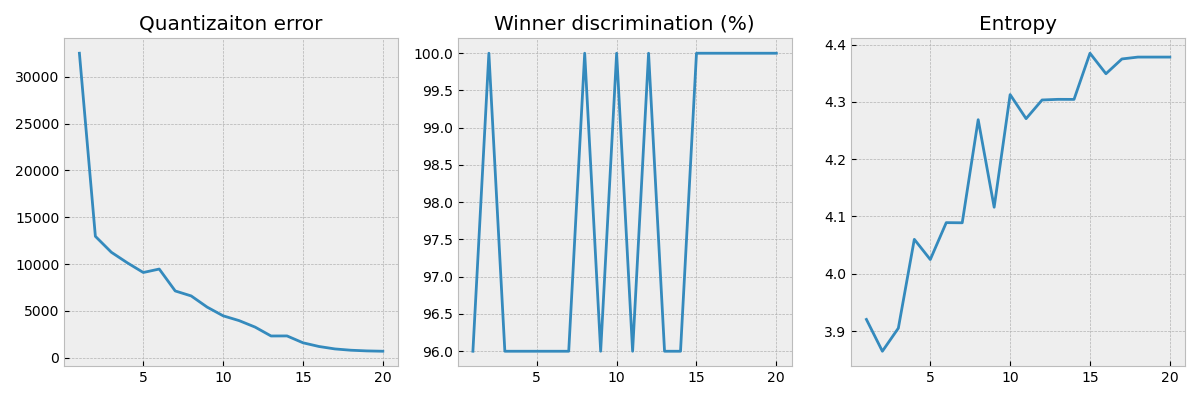
\includegraphics[width=1\textwidth]{figs/som-stats.png}
    \caption{SOM metrics during training}
    \label{fig:som-metrices}
\end{figure}


\subsection{Wine experiment results}

In each experiment, we focused on the investigation of model metrics for several values of hyperparameter $\kappa$ in different setups (number of epochs, architectures, weight initialization, ramp-up types). We trained each setup $20$ times, and all shown results are means and standard deviations of $20$ training runs of the model with described parameters. The following sections contain graphs with visualizations of metrics during training. Means of $20$ runs are marked as dots (baseline model) or triangles (MLP-SOM model) and standard deviations are marked as vertical lines. 

\subsubsection{Experiment 1 (100 epochs)}

In this experiment, we trained the baseline and model with different values of hyperparameter $\kappa$ for 100 epochs. Investigated $\kappa$ values were from interval $0$ to $1$. The best-performing model was the MLP-SOM model with $\kappa = 0.9$ with mean test accuracy $84.67 \pm 10.40$. The baseline had a mean test accuracy of $82.11	\pm 16.08$. In figure \ref{exp1-graphs} we have shown training and testing progress plots of baseline and best-performing model. Training and test metrics of all investigated setups are displayed in table \ref{exp1-res-table}.


\begin{table}[h!]
\centering
\begin{tabular}{|l|l|l|}
\hline
$\kappa$        & training loss & test accuracy (\%) \\ \hline
\color{purple} $0$   &  \color{purple}  $0.062	\pm 0.074 $  & \color{purple}  $82.11	\pm 16.08$  \\ \hline
$0.2$ &   $0.054	\pm 0.062 $  &  $84.00	\pm 10.74$  \\ \hline
$0.3$ &   $0.063	\pm 0.069 $  &  $81.56	\pm 13.84$  \\ \hline
$0.4$ &   $0.082	\pm 0.087 $  &  $77.89	\pm 19.21$  \\ \hline
$0.5$ &   $0.083	\pm 0.086 $  &  $75.22	\pm 19.22$  \\ \hline
$0.7$ &   $0.064	\pm 0.072 $  &  $83.44	\pm 15.37$  \\ \hline
$0.8$ &   $0.089	\pm 0.090 $  &  $75.89	\pm 20.84$  \\ \hline
\color{purple} $0.9$ &  \color{purple}  $0.058	\pm 0.058 $  & \color{purple}  $84.67	\pm 10.40$  \\ \hline
$1$   &   $0.068	\pm 0.061 $  &  $82.67	\pm 11.98$  \\ \hline
\end{tabular}
\caption{MLP-SOM model training results after 100 epochs}
\label{exp1-res-table}
\end{table}


\begin{figure}[h!]
    \centering
    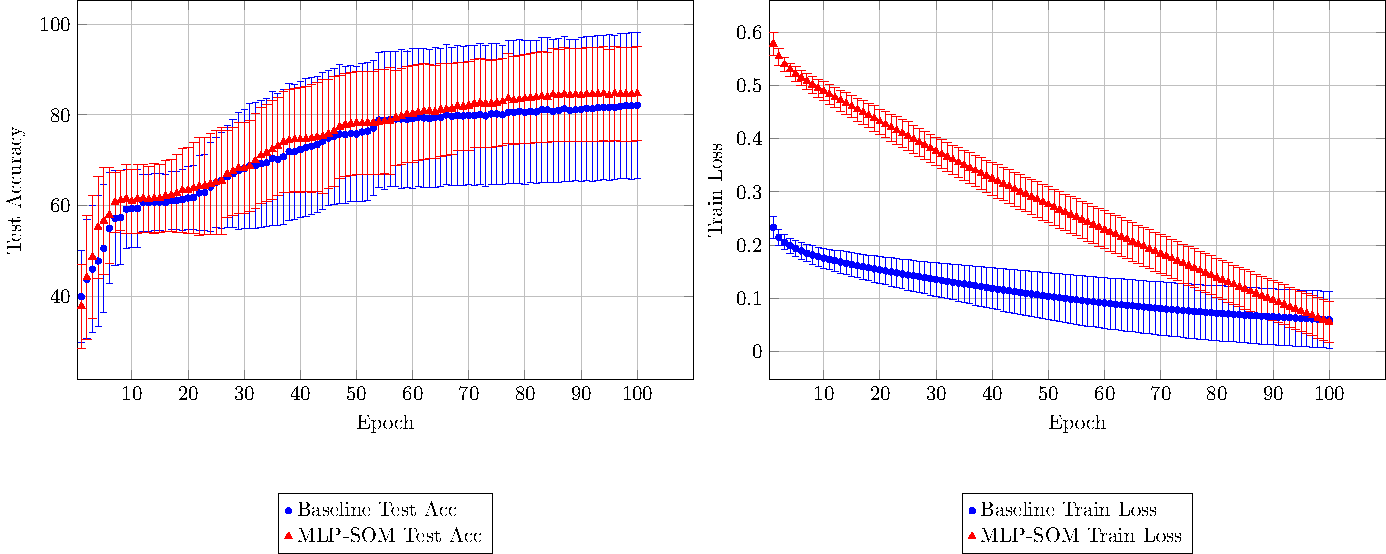
\includegraphics[width=0.9\textwidth]{figs/baseline-model-tr-test-metrices-15hid-100eps-0.9k.pdf}
    \caption{Comparison of training and testing progress plots, 100 epochs, $\kappa$ 0.9}
    \label{exp1-graphs}
\end{figure}

The difference between the test accuracies of the baseline and model indicates that SOM supported the supervised model to produce better predictions. From the metrics graph \ref{exp1-graphs} we can see, that test accuracies change in time looks similar for both models. The baseline has a higher standard deviation. In case of loss, for the MLP-SOM model, it decreases faster than for the baseline model. The trend of the model's loss indicates that it is able to continue to decrease, if we continue training for more epochs. Based on this observation, the next experiment investigated similar setups for 500 epochs. The experiment was run for values of $\kappa$ that performed well in this experiment.

\subsubsection{Experiment 2 (500 epochs)}
In this experiment, we trained models with $\kappa$ values $0.2$, $0.7$, $0.9$ and $1$. Again, the best-performing model had $\kappa = 0.9$. Metrics of this model are shown in figure \ref{exp2-graphs}. The progress plots look quite similar to the previous experiment and the final accuracy is higher for both models. Losses are lower in comparison to 100 epoch training. MLP-SOM model still has better performance than the baseline, it is more than $2.5\%$ better.

\begin{table}[h!]
\centering
\begin{tabular}{|l|l|l|}
\hline
$\kappa$        & training loss & test accuracy (\%) \\ \hline
\color{purple}$0$   &  \color{purple} $0.042	\pm 0.066 $  &  \color{purple} $84.00	\pm 13.18$  \\ \hline
$0.2$ &   $0.038	\pm 0.079 $  &  $84.33	\pm 15.77$  \\ \hline
$0.7$ &   $0.038	\pm 0.079 $  &  $83.89	\pm 16.49$  \\ \hline
\color{purple} $0.9$ &  \color{purple} $0.029	\pm 0.059 $  & \color{purple} $86.78	\pm 11.62$  \\ \hline
$1$   &   $0.047	\pm 0.090 $  &  $82.78	\pm 19.56$  \\ \hline
\end{tabular}
\caption{MLP-SOM model training results after 500 epochs}
\label{exp2-res-table}
\end{table}


\begin{figure}[h!]
     \centering
     \begin{subfigure}[b]{0.49\textwidth}
         \centering
         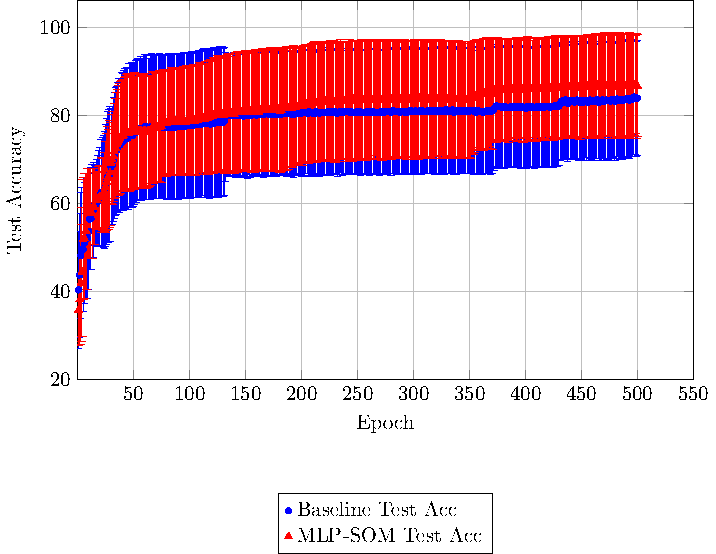
\includegraphics[width=\textwidth]{figs/baseline-model-tr-test-metrices-500-test.pdf}
     \end{subfigure}
     \hfill
     \begin{subfigure}[b]{0.49\textwidth}
         \centering
         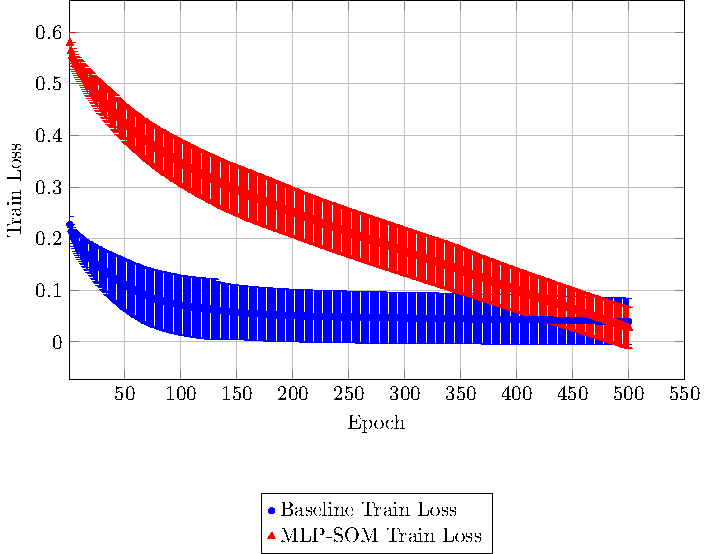
\includegraphics[width=\textwidth]{figs/baseline-model-tr-test-metrices-500-tr.pdf}
     \end{subfigure}
        \caption{Comparison of training and testing progress plots, 500 epochs, $\kappa$ 0.9}
        \label{exp2-graphs}
\end{figure}

\newpage
\subsubsection{Experiment 3 (10 hidden neurons, 250 epochs)}

In this experiment, we focused on an even smaller baseline and MLP-SOM architecture. The new architecture contained one hidden layer with only $10$ neurons. Architecture is described in table \ref{mlp=layers=small}. 

\begin{table}[ht]
    \centering
    \begin{tabular}{ |c|c|c|} 
     \hline
            Layer & Number of neurons & Activation function\\
            \hline
            input fully connected & 13 &  - \\
            \color{purple} hidden fully connected & \color{purple} 10 & sigmoid  \\
            output fully connected  & 3 & softmax \\
     \hline
    \end{tabular}
    \caption{Smaller architecture of MLP}
    \label{mlp=layers=small}
\end{table}

Training a and test metrics are shown in table \ref{exp3-res-table}. The best-performing model has accuracy on the test set $76.11	\pm 19.76$ and hyperparameter $\kappa = 0.7$. The baseline has accuracy of $69.78	\pm 23.9$. Again, the MLP-SOM model has better performance, difference is approximately $6.3\%$. We can see, that both, the baseline and model with combined loss has worse accuracy than in previous experiments. It is probably caused by smaller architecture. Figure \ref{exp3-graphs} shows progress plots of MLP-SOM with $\kappa = 0.7$ and baseline.



\begin{table}[h!]
\centering
\begin{tabular}{|l|l|l|}
\hline
$\kappa$  & training loss & test accuracy (\%) \\ \hline
\color{purple}$0$ & \color{purple}  $0.093	\pm 0.107 $  & \color{purple} $69.78	\pm 23.9$  \\ \hline
$0.1$ &   $0.096	\pm 0.113 $  &  $68.89	\pm 25.89$  \\ \hline
$0.2$ &   $0.074	\pm 0.099 $  &  $74.56	\pm 21.74$  \\ \hline
$0.3$ &   $0.087	\pm 0.102 $  &  $71.56	\pm 22.96$  \\ \hline
\color{purple}$0.7$ & \color{purple}  $0.069	\pm 0.091 $  & \color{purple} $76.11	\pm 19.76$  \\ \hline
$0.9$ &   $0.065	\pm 0.098 $  &  $73.22	\pm 20.91$   \\ \hline
\end{tabular}
\caption{Training results after 250 epochs}
\label{exp3-res-table}
\end{table}

\begin{figure}[h!]
    \centering
    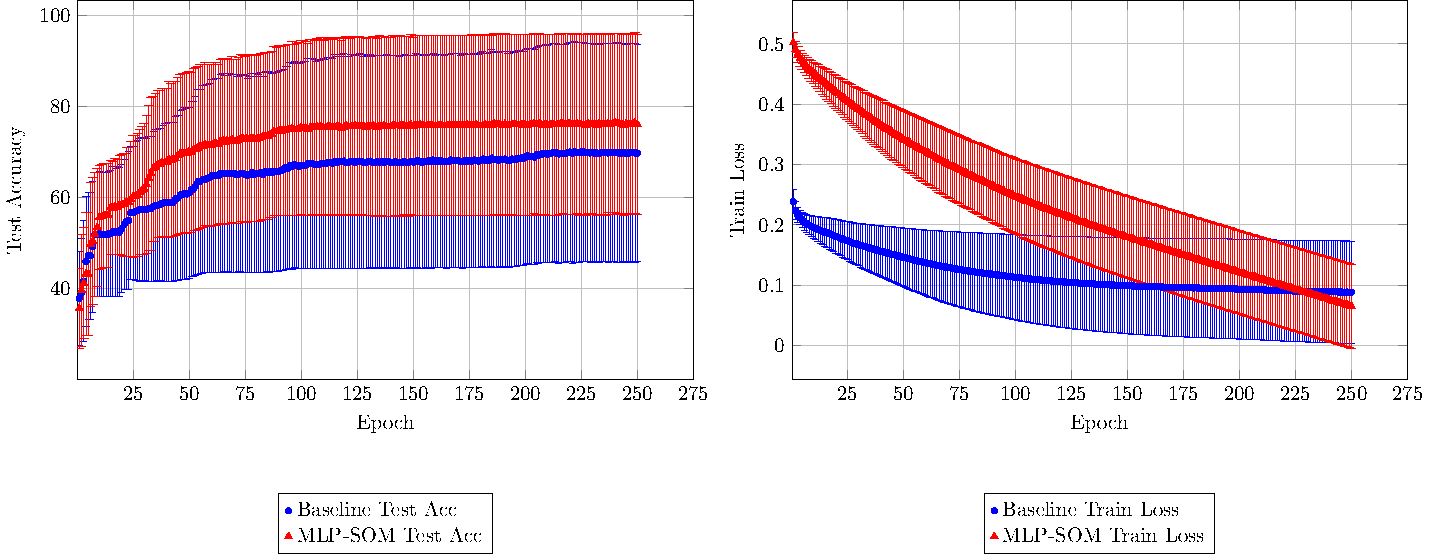
\includegraphics[width=0.8\textwidth]{figs/baseline-model-tr-test-metrices-small-250ep.pdf}
    \caption{Comparison of training and testing progress plots, 250 epochs, $\kappa$ 0.7, 10 hidden neurons}
    \label{exp3-graphs}
\end{figure}


\newpage
\subsubsection{Experiment 4 (weight initialization)}

In all previous experiments, we used default PyTorch weight initialization in the input and hidden layer. In this experiment, we wanted to check, whether different weight initialization improves performance.

Default PyTorch weight initialization for the fully connected layer (linear layer in PyTorch) is from the Kaiming He probability density function with parameter $a = \sqrt{5}$. PyTorch documentation says, that this is equivalent to uniform distribution $U(\frac{-1}{\sqrt{d_{in}}}, \frac{1}{\sqrt{d_{in}}})$, where $d_{in}$ means a number of input features (for our dataset, it is $13$).

We compared this default initialization with initialization from Gaussian (normal) distribution with parameters $\mu = 0$ and $\sigma = 0.2$, marked $N(0, 0.2)$. From the table \ref{exp4-res-table} of results, we can see, that all models with weights initialized from normal distribution had worse performance than ones that were initialized using default PyTorch weight initialization. 


\begin{table}[h!]
\centering
\begin{tabular}{|l|l|l|}
\hline
$\kappa$        & PyTorch init & $N(0, 0.2)$ init \\ \hline
$0$   &  $82.11	\pm 16.08$ &  $78.56	\pm 18.52$ \\ \hline
$0.2$ &  $84.00	\pm 10.74$ &  $78.00	\pm 19.14$  \\ \hline
$0.3$ &  $81.56	\pm 13.84$ & \color{purple} $80.56	\pm 15.84$  \\ \hline
$0.7$ &  $83.44	\pm 15.37$ &  $77.11	\pm 18.67$  \\ \hline
$0.9$ &  \color{purple} $84.67	\pm 10.40$ &  $75.67	\pm 16.89$  \\ \hline
$1$   &  $82.67	\pm 11.98$ &  $78.56	\pm 18.64$   \\ \hline

\end{tabular}
\caption{Test accuracy after 100 epochs}
\label{exp4-res-table}
\end{table}


\subsubsection{Experiment 5 (non-linear $\kappa$ ramp down)}

Since we introduced parameter $\kappa$ for the ratio of $J_S$ in combined loss and used it in setup when it is linearly ramped down in this experiment we study other possible forms of parameter ramping. Linear ramp down for different values is shown in Fig.\ref{fig:ramps} on the left and the definition of $\kappa(t)$ is in equations \ref{eq-t} and \ref{eq-linear-ramp}.

\begin{equation}
    t = \frac{current\ epoch}{total\ epochs}
    \label{eq-t}
\end{equation}

\begin{equation}
    \kappa(t) = \kappa \cdot (1 - t) 
    \label{eq-linear-ramp}
\end{equation}

We tried two other types of ramps, sigmoid ramp down (Fig.\ref{fig:ramps} in the middle) and combined sigmoid ramp up and sigmoid ramp down (Fig.\ref{fig:ramps} on the right). sigmoid ramp down was inspired by a ramp in implementation of the Mean Teacher model \cite{curiousai}. Value of $kappa(t)$ was set based on equation \ref{eq-sigm-ramp}. We study also combined sigmoid ramp up and sigmoid ramp down and $kappa(t)$ was set as in equation \ref{eq-comb-ramp}.

\begin{equation}
    \kappa(t) = \kappa \cdot e^{-5 \cdot t^2}
    \label{eq-sigm-ramp}
\end{equation}

\begin{equation}
    \kappa(t) = \begin{cases}
		      \kappa \cdot e^{-5  (1-5t)^2}, & \text{if $t < \frac{1}{5}$ }\\
            \kappa, & \text{if $\frac{1}{5} \leq t < \frac{1}{3}$}\\
            \kappa \cdot e^{-5  (\frac{3t - 1}{2})^2}, & \text{if $t < \frac{1}{5}$ }
		 \end{cases}
    \label{eq-comb-ramp}
\end{equation}




\begin{figure}[h!]
    \centering
    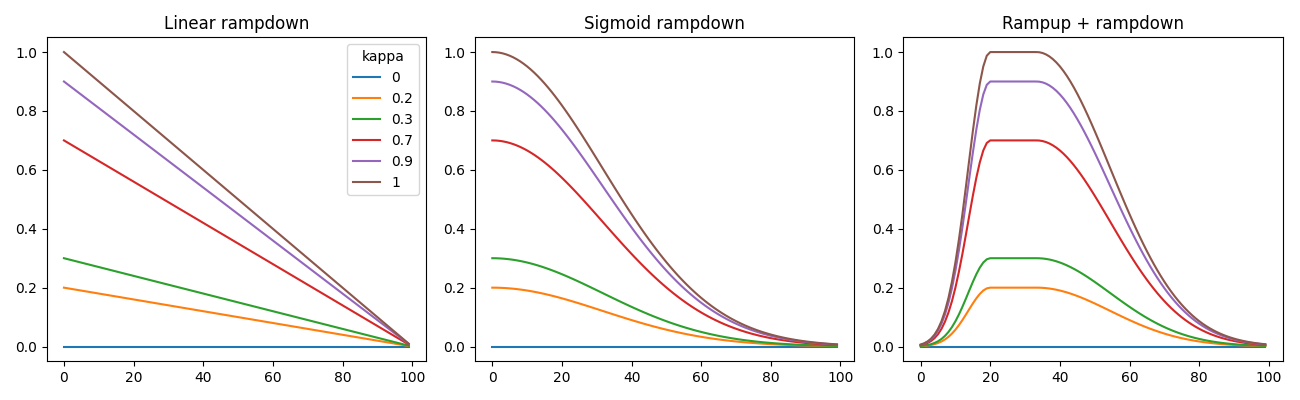
\includegraphics[width=1\textwidth]{figs/ramps.png}
    \caption{Visualisation of ramp types for used values of $\kappa$}
    \label{fig:ramps}
\end{figure}

\begin{table}[h!]
\centering
\begin{tabular}{|l|l|l|l|}
\hline
$\kappa$        & linear ramp down & sigmoid ramp down & ramp up + ramp down \\ \hline
$0$   &  \color{purple} $82.11	\pm 16.08$ &                         &  \\ \hline
$0.2$ &  $84.00	\pm 10.74$ &  $85.11	\pm 14.73$   &  $80.89	\pm 16.59$ \\ \hline
$0.3$ &  $81.56	\pm 13.84$ &  $85.33	\pm 11.38$   &  $79.78	\pm 18.2$  \\ \hline
$0.7$ &  $83.44	\pm 15.37$ & \color{purple} $89.22	\pm  6.53$   &  $79.89	\pm 14.25$ \\ \hline
$0.9$ &  $84.67	\pm 10.40$ &  $77.89	\pm 18.59$   &  $74.78	\pm 19.17$ \\ \hline
$1$   &  $82.67	\pm 11.98$ &  $79.11	\pm 16.61$   &  $78.44	\pm 18.62$ \\ \hline

\end{tabular}
\caption{Test accuracy after 100 epochs}
\label{exp5-res-table}
\end{table}


From the table of results, we can see, that the overall best-performing model used the sigmoid ramp-down function and $\kappa$ hyperparameter set to $0.7$. This model has a test accuracy of $89.22	\pm  6.53$. The baseline model is the same for all types of ramps, because when $\kappa = 0$, then for all t $\kappa(t)$ is also equal to zero. This holds for all three ramp types. Baseline model accuracy is $82.11	\pm 16.08$, so the MLP-SOM model is $7\%$ better than the baseline. 

We can see, that combined ramp has worse results than linear and sigmoid ramps. sigmoid ramps work better for smaller values of $\kappa$ and for values $0.2$ and $0.3$ has better results than linear ramp. In case of higher $\kappa$ values, the linear ramp worked better.


\subsection{Zoo experiment results}
As another step of our experimentation, we tried to reproduce MLP-SOM model performance with different dataset. We chose a dataset called Zoo Animal dataset. It is tiny table dataset with a description of animals from $7$ categories. Each sample is described by $16$ boolean or integer attributes. There are $101$ samples in the dataset. We divided samples into test and train sets. The test set contained $2$ samples from each category, so it was composed of $14$ samples. The rest of the samples were used to create $7830$ triplets - training dataset.

We pre-trained SOM with training data for $50$ epochs. The map is shown in figure \ref{fig:som-zoo}. We can see, that half of the neurons were never chosen as winners, which corresponds to the winner discrimination metric. The other two metrics - entropy and quantization error - had correct increasing and decreasing trends.

\begin{figure}[h!]
    \centering
    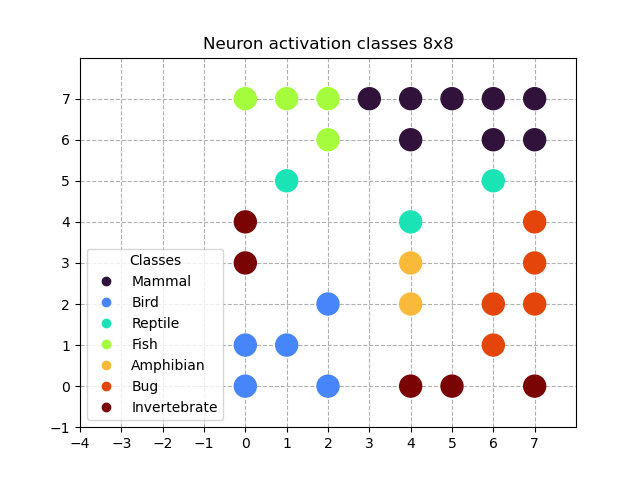
\includegraphics[width=0.9\textwidth]{figs/som1710884692.939712.png}
    \caption{Pre-trained SOM map after 50 epochs}
    \label{fig:som-zoo}
\end{figure}


In this experiment, we tried all promising $\kappa$ values, both weight initialization methods and linear and sigmoid ramps. Table of results \ref{tab:zoo} shows mean and standard deviations of $10$ models for each combination of hyperparameters. The baseline has the test accuracy of $92.14\pm 2.14$. We can see, that any model with a sigmoid ramp has worse accuracy than baseline. We can also see, that all of the models with linear ramp have at least that good accuracy as the baseline. The highest accuracy has the model with $\kappa = 0.75$ and Gaussian weight initialization, however, it has quite a high standard deviation compared to the baseline. We can see, that a model with $\kappa = 0.75$ and PyTorch weight initialization, the same as a model with $\kappa = 0.5$ and Gaussian weight initialization, has accuracy $93.57\pm 2.14$, which is the same standard deviation as in baseline and the difference of means is almost $1.5\%$.

\begin{table}[h!]
\centering
\begin{tabular}{|c|cc|cc|}
\hline
     & \multicolumn{2}{c|}{linear ramp} & \multicolumn{2}{c|}{sigmoid ramp} \\ \hline
 & \multicolumn{1}{c|}{PyTorch init} & $N(0, 0.2)$ init & \multicolumn{1}{c|}{PyTorch init} & $N(0, 0.2)$ init \\ \hline
base  & \multicolumn{1}{c|}{$92.14\pm 2.14$}    &   $92.14\pm 2.14$   & \multicolumn{1}{c|}{}      &       \\ \hline
0.25  & \multicolumn{1}{c|}{$92.86\pm 0.00$}     &   $93.57\pm 3.85$   & \multicolumn{1}{c|}{$80.0	\pm 2.86$}      &  $81.43\pm 3.50$     \\ \hline
 0.5  & \multicolumn{1}{c|}{$92.86\pm 0.00$}     &   $93.57\pm 2.14$   & \multicolumn{1}{c|}{$80.0	\pm 2.86$}      &  $79.29\pm 2.14$    \\ \hline
0.75  & \multicolumn{1}{c|}{$93.57\pm 2.14$}    &  $94.29\pm 2.86$    & \multicolumn{1}{c|}{$81.43	\pm 3.50$}      &   $80.71\pm 4.57$    \\ \hline
   1  & \multicolumn{1}{c|}{$93.57	\pm 2.14$}   &  $92.14\pm 2.14$    & \multicolumn{1}{c|}{ $80.71	\pm 3.27$}      &   $82.14	\pm 3.57$     \\ \hline

\end{tabular}
\caption{Table of Zoo experiment results, test accuracy of models after 200 epochs}
\label{tab:zoo}
\end{table}

\section{Implementation}
This experiment was implemented using PyTorch library \cite{pytorch}. The implementation of SOM was adapted from this repository \cite{som-repo}. Experiment implementation is available in our GitHub repository \cite{dt-mt-repo}. It can be found in folder \\ \texttt{pytorch/experiments/som-loss-developement}. File \texttt{dataset.py} is shared for the Wine and Zoo experiment. In sub-folders \texttt{wine} and \texttt{zoo}, the source code of MT-SOM models and pre-training of SOM with proper size and input dataset are placed. 

\section{Discussion}
In this chapter, we show that SOM-based auxiliary information can help in the training of supervised Multi-layer perceptron. We proved our concept of the MLP-SOM model on two datasets. For each dataset, experiments show, that the test accuracy of MLP-SOM is better than the accuracy of vanilla Multi-layer perceptron with the same architecture. Based on these results, we have a strong belief, that SOM topology information as an auxiliary loss will help also in semi-supervised setup.